\documentclass{article}

% -------------------------------------------- usepackage  -------------------------------------------- %
\usepackage[utf8]{inputenc}
\usepackage[english]{babel}
\usepackage[T1]{fontenc}
\usepackage{amsmath,amssymb,amsfonts,amsthm}
\usepackage{ulem}
\usepackage{subcaption}
\usepackage{caption}
\usepackage{gauss}
\usepackage{mathtools}
\usepackage{mathrsfs}
\usepackage{hyperref}
\usepackage{bbm}
\usepackage{graphicx} 
\usepackage{enumerate} 
\usepackage{fancyhdr} 
\usepackage{lastpage} 
\usepackage[margin=1in,footskip=0.25in]{geometry}
\usepackage{pdfpages}
\usepackage{pdfpages}
\usepackage{bookmark}

% -------------------------------------------- newcommand  -------------------------------------------- %
\pagestyle{fancy}
\setcounter{MaxMatrixCols}{20}
\linespread{1,2}
\newcommand{\pic}[3]{\makebox[\textwidth]{\textbf{#1}}
\\
\begin{center}
\includegraphics[scale=#2,center]{#3}
\end{center}}
\newcommand{\QQ}{\mathbb{Q}}
\newcommand{\RR}{\mathbb{R}}
\newcommand{\BB}{\mathbb{B}}
\newcommand{\NN}{\mathbb{N}}
\newcommand{\FF}{\mathbb{F}}
\newcommand{\ZZ}{\mathbb{Z}}
\newcommand{\CC}{\mathbb{C}}
\newcommand{\EE}{\mathbb{E}}
\newcommand{\indi}[1]{\mathbbm{1}_{#1}}
\newcommand{\limi}[2]{\liminf\limits_{#1\rightarrow#2}}
\newcommand{\bcup}[1]{\bigcup\limits_{#1}}
\newcommand{\bcap}[1]{\bigcap\limits_{#1}}
\newcommand{\m}{\cdot}
\newcommand{\ver}[2]{#1\hspace{0.05cm}\vert\hspace{0.03cm}#2}
\newcommand{\mgd}[2]{\left\{#1 \hspace{0.1cm}\left|\hspace{0.1cm}#2\right.\right\}}
\newcommand{\ls}{\limsup\limits_{n\rightarrow\infty}}
\newcommand{\li}{\liminf\limits_{n\rightarrow\infty}}
\newcommand{\Part}[2]{\frac{\partial{#1}}{\partial{#2}}}
\newcommand{\Int}[4][x]{\int_{#2}^{#3} #4 \hspace{0.05cm}\mathrm{d} #1}
\newcommand{\myeq}[2][=]{\mathrel{\overset{\makebox[0pt]{\mbox{\normalfont\tiny\sffamily $#2$}}}{#1}}}
\newcommand{\Myeq}[2][\leq]{\mathrel{\overset{\makebox[0pt]{\mbox{\normalfont\tiny\sffamily $#2$}}}{#1}}} 
\newcommand{\mb}[1]{\mathbb{#1}}
\newcommand{\mc}[1]{\mathcal{#1}}
\newcommand{\ms}[1]{\mathscr{#1}}
\newcommand{\as}{\myeq[\rightarrow]{as}}
\newcommand{\As}{\myeq[\sim]{as}}
\newcommand{\wk}{\myeq[\rightarrow]{wk}}
\newcommand{\Pkonv}{\myeq[\rightarrow]{P}}
\newcommand{\Dkonv}{\myeq[\rightarrow]{D}}
\newcommand{\Lkonv}[1][1]{\myeq[\rightarrow]{\mc{L}^{#1}}}
\newcommand{\inte}[3]{\int_{#1} #2 \hspace{0.05cm}\mathrm{d}{#3}}
\newcommand{\Norm}[1]{\left\lVert#1\right\rVert}
\newcommand{\norm}[1]{\left\lvert#1\right\rvert}
\newcommand{\Sum}[2]{\sum\limits_{#1}^{#2}}

% -------------------------------------------- document  -------------------------------------------- %
\title{}
\author{}
\makeatletter
\providecommand*{\cupdot}{%
  \mathbin{%
    \mathpalette\@cupdot{}%
  }%
}
\newcommand*{\@cupdot}[2]{%
  \ooalign{%
    $\m@th#1\bigcup$\cr
    \hidewidth$\m@th#1\cdot$\hidewidth}%
}
\makeatother



\begin{document}

% -------------------------------------------- import files  -------------------------------------------- %
% import the front page
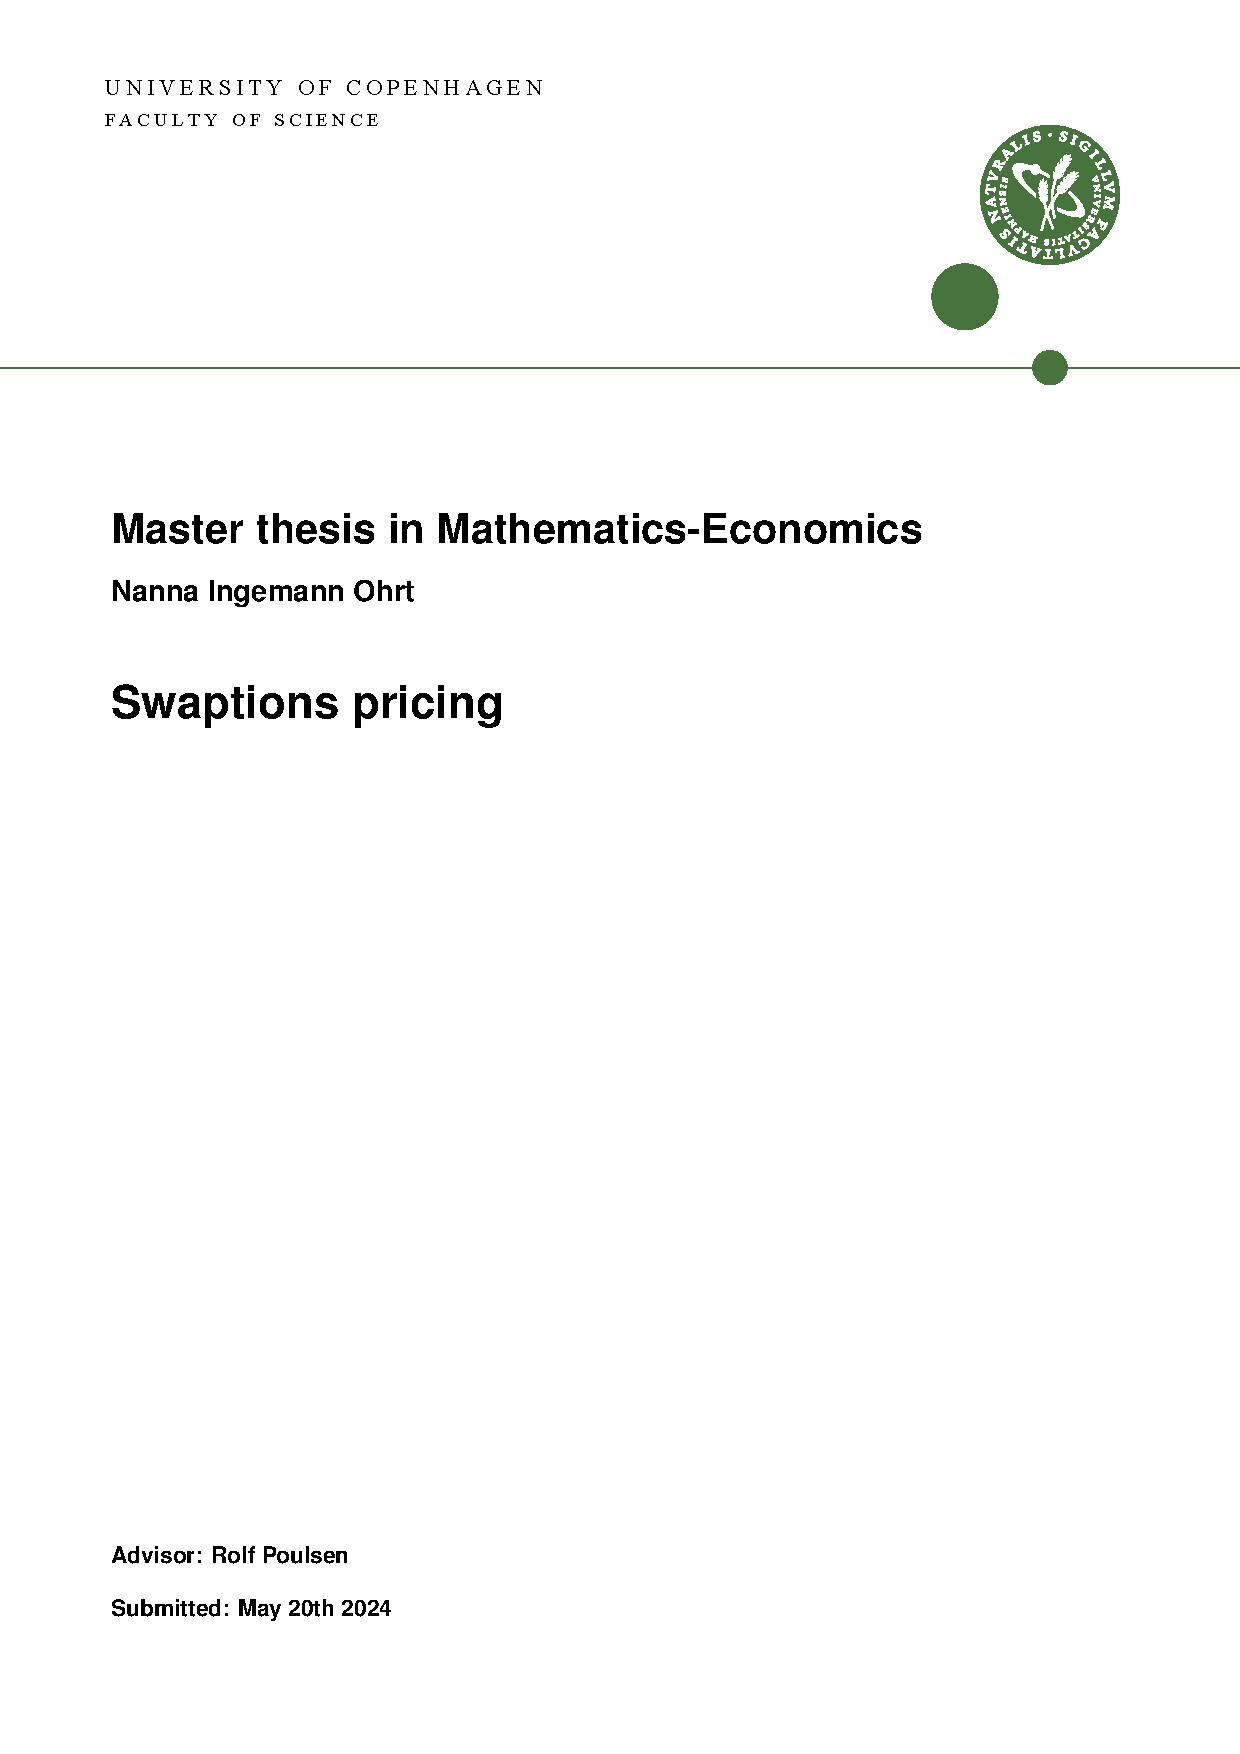
\includepdf[pages=-]{/Users/nannaingemannohrt/Desktop/master_thesis/main/frontpage/frontpage_setup.pdf} 

% import the abstract
\section*{Abstract}

Hej Rikke
\newpage

% make table of contents
\tableofcontents 

\newpage
\section{Introduction}




\begin{tikzpicture}[node distance=1cm and 1cm, auto]
  % Nodes
  \node (t0) {Time 0};
  \node[below= of t0] (t1) {Time 1};
  \node[below= of t1] (t2) {Time 2};
  \node[below= of t2] (t3) {Time 3};
  \node[below= of t3] (t4) {Time 4};
  
  % Arrows
  \draw[-Latex] (t0.south) to [bend right] node[left] {forward} (t1.north);
  \draw[-Latex] (t1.south) to [bend right] node[left] {forward} (t2.north);
  \draw[-Latex] (t2.south) to [bend right] node[left] {forward} (t3.north);
  \draw[-Latex] (t3.south) to [bend right] node[left] {forward} (t4.north);
  
  \draw[-Latex] (t1.north) to [bend right] node[right] {back} (t0.south);
  \draw[-Latex] (t2.north) to [bend right] node[right] {back} (t1.south);
  \draw[-Latex] (t3.north) to [bend right] node[right] {back} (t2.south);
  \draw[-Latex] (t4.north) to [bend right] node[right] {back} (t3.south);

  % Dotted lines
  \draw[dotted] (t4.south) -- ++(0,-1cm);
  \draw[dotted] (t0.north) -- ++(0,1cm);
  
\end{tikzpicture}


\newpage  

\clearpage
\addcontentsline{toc}{section}{References}

\begin{thebibliography}{25}
 \bibitem{Bjork}
 Björk, Tomas,
 \emph{Arbitrage Theory in Continuous Time},
 Oxford, fourth edition, 2020

 \bibitem{Hull}
Hull, John C., 
\emph{Options, futures, and other derivatives},
Pearson, eleventh edition, global edition, 2022

\bibitem{Lindstrøm}
Linderstrøm, Martin Dalskov, 
\emph{Fixed Income Derivatives Lecture Notes},
2013
 
\end{thebibliography}

\bibliography{tesis} 
\section{Swaptions as a missing link in asset allocation}


\section{Mathematics of pricing swaptions}
To determine swaptions prices, it is important to understand which things there affects the price of the swaption. 
This chapter simplifies these concepts by explaining interest rates, bonds, swaps, and options, 
and then shows how they come together to determine the price of a swaption.
\subsection{Time value of money}
Understanding the concept of interest rates begins with the fundamental idea that a dollar today holds 
more value than the same dollar in the future. To understand these concept, a discount factor is introduce 
\begin{align*}
    B(t,T) = \text{value at time t of a dollar received at time T}
\end{align*} 
$B(t,T)$ refer to a contract that pays one dollar maturity, T, which can be illustrated as below
\begin{align*}
    t & < T \rightarrow B(t,T) < 1 \\
    t & = T \rightarrow B(t,T) = 1
\end{align*}
The concept "time value of money" it asserts that the value of money today is worth more than
the same amount in the future due to its potential earning capacity, inflation, and risk.
This principle underpins various financial decisions, including investing, borrowing,
and pricing financial instruments. Essentially, it recognizes that a dollar received today can be invested 
and earn interest over time, thereby increasing its value. Conversely, a dollar received in the future
is subject to uncertainty and may not retain its purchasing power due to inflation or other factors.
The discount factor represents the present value of future cash flows, taking into account the time value of money.
It reflects the idea that receiving a certain amount of money in the future is less valuable than receiving 
the same amount today.
\subsection{Zero coupon bonds}
One of the most common applications of the concept "time value of money" is zero coupon bonds. 
By there construction the mechanism of "time value of money" is present. This instrument 
have the common property that they provide the owner with a deterministic cash flow. 
\begin{definition}\label{def:zcb}
    A zero coupon bond with maturity data T, also called a T-bons, is a contract which 
    guarantees the holder one dollar to be paid on the date T. The price at time t of 
    a bond with maturity data T is denoted by p$(t,T)$ \cite{Bjork} 
\end{definition} 
\subsection{The yield curve}
Where the concept "time value of money" and the discount factor are fundamental concepts used to assess the present value of future
cash flows, while the yield curve provides insights into market expectations regarding future interest rates.
Understanding the interplay between these concepts is crucial for making informed investment decisions and pricing
financial instruments. The yield curve is a graphical representation illustrating the interest rates (bond yields) for various maturities.
Yield curve can provide a intuition about future interest rates and give insight in the bond market today. 
The general intuition is that longer-term rates is higher then short-term rates, which in other words means that a
lager premium is expect for lending money over a longer period of time. This case sketches a yield cure with a 
positive slope.
\subsection{Interest rates}
\subsubsection{Spot rates}
The spot rate represents the yield-to-maturity of a zero coupon bond,
while the forward rate refers to the anticipated interest rate in the 
future. The definition for determined spot rates is listed 
below
\begin{definition}\label{def:spot}
    The simple spot rate for $[S,T]$, henceforth referred to as the 
    LIBOR spot rate, is defined as \cite{Bjork} 
    \begin{align*}
        L(t;S,T) = - \frac{p(t,T)-p(t,S)}{(T-S)p(t,T)}
    \end{align*}
\end{definition} 
\subsubsection{Forward rates}
Forward rates play a crucial role in financial markets, particularly in the realm of interest rate analysis and 
derivative pricing. They represent the interest rate applicable to a future period, agreed upon today.
Understanding forward rates requires grasping the concept of forward contracts and the expectations theory of interest rates.
Forward rates can be derived from the yield curve. The yield curve plots the yields of bonds with different maturities.
By analyzing the yield curve, one can infer the implied forward rates for future periods. For example, 
the forward rate between year 1 and year 2 is the rate at which an investor can borrow or lend money for the period
between year 1 and year 2, starting at year 1.
\\\\
Lets consider three time points on the yield curve $t=0,1,2$, where it is assumed
that $t_0 < t_1 < t_2$. At time $t_0$ we have the spot rates $p(t_0,t_1)$ and $p(t_1,t_2)$,
which represent the yields for bonds maturing at time $t_1$ and $t_2$ respectively.
Hence the forward rate, $R(t_1,t_2)$, can med determined using the equation below
\begin{align*}
    R(t_1,t_2)= \frac{(1+p(t_0,t_2))^2}{(1+p(t_0,t_1))}-1
\end{align*}
Imagine investing one dollar in a one-year zero-coupon bond, $B(t_0,t_1)$,
and instantly reinvesting the money received at time $t_1$ in a new one-year zero-coupon bond,
$B(t_1,t_2)$, at rate $R(t_1,t_2)$. This strategy should yield the same return as investing 
one dollar in a two-year zero coupon bond $B(t_0,t_2)$ and holding it for two years. 
This strategy illustrated the idea of forward rates. Let us then look a the general
formula for forward rates. 
\begin{definition}\label{def:forward}
    The continuously compounded forward rate for $[S,T]$ contracted at t is defined
    as \cite{Bjork} 
    \begin{align*}
        R(t;S,T)= - \frac{\log p(t,T)- \log p(t,S)}{(T-S)} 
    \end{align*}
\end{definition} 
\subsection{Financial derivatives}
\subsubsection{Bonds}
A bond is a debt security, like a loan. Borrowers issue bonds to raise money 
from investors willing to lend them money for a certain amount of time.
When you purchase a bond you are lending money to the issuer, which in 
some cases is a government or company. In return, from the construction of the 
bond, the issuer guarantees to pay a predetermined rate during the term of the bond
and repay the principal at maturity. 
\\\\
Earlier a zero coupon bond has ben introduced and when talk about bonds, a zero coupon 
bond is the simplest representation of a bond. The zero coupon bond contract is 
only given by two cash flows. One for the buyer, there pays the issuer at time 
t = $t_0$, and another where the buyer receives the principal at time t = T.
Unlike other types of bonds, a zero coupon bond does not offer periodic 
interest payments (coupons) throughout its term. \cite{Bjork} 
\\\\
The price of a zero coupon bond is represented as 
p(t,T), where an individual lends an amount, K, with the intention of earning a
return in the future. Therefore, the price of a zero coupon bond, with 
its principal (also known as face value) K, at time t and with maturity 
T, is denoted as.
\begin{align*}
    p(t,T)= B(t,T)\cdot K
\end{align*}
\subsubsection{Fixed Coupon Bonds}
As describe a zero coupon bond does not involve coupons throughout the term of the bond. 
But moving forward we will introduce various bond with coupon there are either fixed 
or floating. First we will consider the simplest form of a coupon bond, which is a 
fixed coupon bond. Fixed coupon bonds are a type of debt security that offers investors a predictable
return in the form of regular interest payments, known as coupons, until the bond's maturies.
These coupons are set at a fixed rate at the time of issuance, based on the bond's face value,
and are typically paid annually or semi-annually. Upon reaching maturity, the issuer repays 
the principal amount (face value) to the issuer, concluding the bond contract. The purpose
of a fixed coupon bond is there ability to provide a steady stream of income,
making them an attractive option for conservative investors seeking to minimize risk and 
secure predictable returns.
\\\\
Continuing we will compute the price of a fixed coupon bond. First we note that the fixed coupon bond,
can be replicated by holding a portfolio consisting of zero coupon bond with maturities $T_i$, for 
$i=1,...,n$. So we will hold $c_i$ zero coupon bonds of maturities $T_i$ for $i=1,...,n-1$, and 
$K+c_n$ bonds with maturity $T_n$. Hence we have that the price, p(t), at time t, where $t<T$, of 
the fixed coupon bonds becomes. \cite{Bjork}
\begin{align*}
    p(t) = K \cdot p(t,T_n) + \sum_{i=1}^{n}c_i \cdot p(t,T_i)
\end{align*}
When taking about coupons, there are typically determined in terms of return than in monetary terms.
So the return of the i'th coupon is denoted as a simple rate acting in the face value K, over the
time period $[t_{i-1},T_i]$. So for the i'th coupon the return is equal to $r_i$, and the face value 
is K, hence we have that 
\begin{align*}
    c_i = r_i(T_i-T_{i-1})K
\end{align*}
Where for standardized coupon, the time intervals will be equally spaced, which means that 
\begin{align*}
    T_i = T_0 + i \delta
\end{align*}
This also means the the coupon rates $r_1,...,r_n$ will be equal to a common coupon rate r. 
Hence the price p(t,T) of a fixed coupon bond where $t \leq T_1$ will be determined as below \cite{Bjork}
\begin{align*}
    p(t)= K \Big( p(t,T_n)+ r \delta \sum_{i=1}^{n}\cdot p(t,T_i) \Big)
\end{align*}
\subsubsection{Floating Rate Bonds}
Now a short introduction to fixed coupon bonds has be given, as mentioned there are also many 
type of bonds there have floating coupon. When it is listed that there are bonds there have
floating coupon, what there is really said is that the rate is floating. So with the fixed coupon
bond, the coupon was at predetermined when the agreement was made. But there are also bond, where
the coupon is reset for every coupon period. These types of bond is referred to as floating 
rate bonds. The most simple floating rate bond, is where the coupon rate $r_i$ is set to 
the spot LIBOR rate $L(T_{i-1}, T_i)$. Thus we have that 
\begin{align*}
    c_i = (T_i-T_{i-1})L(T_{i-1},T_i)K
\end{align*}
Here we have that $L(T_{i-1},T_i)$ is determined at time $T_{i-1}$, but the coupon is first 
delivered at time $T_i$. \cite{Bjork}  
\\\\
The LIBOR rate stands for London InterBank Offered Rate, which is a rate the the 
British Bankers Association sets every business day. Like the LIBOR rate, there is many types
of xIBOR rates, one is EURIBOR rate Which is a rate the 
European Banking Federation sets every business day. 
\\\\
These different type of xIBOR rates are sets differently, but they all use the money market convention. 
So when taking about business day, the money market convention is important. This is a day-count 
convention is a standardized methodology for calculating the number of days between two dates.
This means that when $t <T_0$  the coupon dates are equally spaced with  
\begin{align*}
    \delta = T_{i}-T_{i-1}
\end{align*}
To determined the value of a the simplest floating rate bond, the LIBOR spot rate we can without
loss is generality assume that K=1 and insert the Definition \ref{def:spot} of the LIBOR spot rate 
to obtain
\begin{align*}
    c_i &= (T_i-T_{i-1})L(T_{i-1},T_i)K \\
        &= \delta L(T_{i-1},T_i) \\
        &= \frac{1- p(T_{i-1},T_i)}{\delta p(T_{i-1},T_i)} = \frac{1}{p(T_{i-1},T_i)}-1
\end{align*}
This lead to a formula for the floating rate bond, which is listed below \cite{Bjork}
\begin{align*}
    p(t)= p(t,T_n) + \sum_{i=1}^{n}\Big[p(t,T_{i-1})-p(t,T_i)\Big] = p(t,T_0)
\end{align*}
where we note that if $t=T_0$ we get that $p(T_0)=1$
\\\\
This leads to some general assumption there guarantee the existence of a sufficiently 
rich and regular bond market
\begin{assumption}\label{def:market}
    We assume the following
    \begin{itemize}
        \item There exists a (frictionless) market for T-bond for every T>0
        \item The relation p(t,t)= 1 holds for all t
        \item For each fixed t, the bond price p(t,T) is differentiable w.r.t time of maturity T \cite{Bjork}
    \end{itemize}
\end{assumption}
\subsection{Interest rate swaps}
Now some simple cases of different type of bonds has be introduce. Then we will combined the knowledge we have gained to move on
to take interest rate derivatives in consideration. Again we will consider the simplest type of a interest rate derivative, which is a
interest rate swap. The construction of a interest rate swap is that there is exchange a payment stream of a fixed rate of interest,
which is know as the swap rate. This fixed rate is exchange for some floating rate, such as the LIBOR rate. 
As mentioned the fixed rate is know as the swap rate, this swap rate is determined from forward rate extracted from the yield curve, 
so it makes the present value of the swap equal to zero. This we will formulate this later. 
\\\\
As stated in the interest rate swap, two cash flow are exchanged, where one of is a 
fixed cash flow and the other is a floating cash flow. These components of
the interest rate swap are known ad the "fixed leg" and the "floating leg". 
The role of each participant in the swap is determined in relation to the 
fixed leg: the party making fixed payments is engaged in a "payer swap," 
while the party making floating payments (and receiving fixed payments) is
 involved in a "receiver swap."
\\\\
Again we have that K is the principal also know as the face value and we will denote the swap rate, R. Further we have that the payments
arises at the dates $T_1,...,T_n$, this means that at time $T_i$ buyer of the interest rate swap will pay
\begin{align}
    K \delta L(T_{i-1},T_i)
    \label{irs}
\end{align}
where we have that $L(T_{i-1},T_i)$ is the spot rate, which could be the LIBOR spot rate.
  It is also assumed
that the days $T_0,...,T_n$ is equally spaced this $\delta = T_i - T_{i-1}$ as mentioned above in the section for floating rate bonds. 
The it is noticed the expression in \autoref{irs} is the same as $Kc_i$, where again $c_i$ is the i'th coupon for the floating rate. 
So at time $T_i$ the buyer will pay $K \delta R$, where the cash flow at time $T_i$ is given by below
\begin{align*}
    K \delta \Big[L(T_{i-1},T_i)-R \Big]
\end{align*}
Then by applying the results from the section for floating rate bonds again, we are able to compute the value of the 
cash flow at time $t<T_0$. The value of the cash flow is listed below
\begin{align*}
    K p(t,T_{i-1})-K(1+\delta R)p(t,T_i)
\end{align*}
Hence we have that the total value denote by $\Pi(t)$, so the total value at time t of the swap is given as below
\begin{align}
    \pi (t) = K \sum_{i=1}^{n} \Big[p(t,T_{i-1})-(1+ \delta R)p(t,T_i)\Big]
    \label{valueirs}
\end{align}
Moving forward we simplify \autoref{valueirs} in the below Proposition \ref{simple} \cite{Bjork}
\begin{proposition}
    The price, for $t<T_0$, of the swap in \autoref{valueirs} above
    is given by 
    \begin{align*}
        \Pi(t) = K p(t,T_0)-K \sum_{i=1}^{n}d_i p(t,T_i)
    \end{align*}
    where
    \begin{align*}
        d_i &= R \delta, \quad i=1,...,n-1 \\
        d_n &= 1+ R \delta
    \end{align*}
    \label{simple}
\end{proposition}
\noindent 
Earlier we left behind a discussion of how the swap rate, R,  is determined. 
It was noted that the swap is determined such that the present value of
the swap is equal to zero. Now we will give a more accurate definition of how swap is determined in Proposition \ref{swaprate1}.
\begin{proposition}
    If, by convention, we assume that the the contract is written at $t=0$, 
    the swap rate is given by \cite{Bjork}
    \begin{align*}
        R = \frac{p(0,T_0)-p(0,T_n)}{\delta \sum_{i=1}^{n}p(t,T_i)}
    \end{align*} 
    \label{swaprate1}
\end{proposition}
\noindent 
If we have that $T_0=0$ the formula for the swap rate, R, becomes
\begin{align*}
    R= \frac{1-p(0,T_n)}{\delta \sum_{1}^{n}p(0,T_i)}
\end{align*}
\subsection{Options}
In this section will introduce the framework of options in the over-the-counter-market. 
The purpose of this section is to establish a pricing formula for European call options.
The meaning of introducing pricing of options before introducing swaptions pricing, is that a swaption is  a 
more complex derivative. So the idea is to get a fundamental understanding of pricing derivatives in a more simple case.
\\\\
Firstly, let's clarify what the over-the-counter market (OTC) is. It is  a marketplace where numerous trades occur.
In the OTC market private companies exchange trades, these companies are firms as banks, other 
large financial institutions and funds managers \cite{Hull}. Then we have establish the market where 
options is traded, so moving further we will look in to options contracts. 
\\\\
A call options gives the holder the right to but the underlying asset at a fixed strike price, K, and a 
predetermined time to maturity, T. Where a put option gives the holder the right to sell the underlying asset at a fixed
strike price, K, and a predetermined time to maturity, T. Options contracts come in various types, with the 
most common being the European and American options, followed by Bermudan options. European options can only 
be exercised at the maturity date, while American options can be exercised at any time point upon to the maturity date.
Bermudan options allow exercise at specific predetermined time points.
For the purpose of understanding the basics of options pricing, we will focus on the European option. 
The contract functions, $\Phi$, for European call and put options are as follows.
\begin{align}
    \Phi(x)_{\text{call}} &=  \max[S-K,0] \label{call_function}\\ 
    \Phi(x)_{\text{put}} &= \max [K-S,0] \label{put_function}
\end{align}
where K is the strike price, S denotes the market price of the underlying asset \cite{Bjork}. From \autoref{call_function} and \autoref{put_function} we see
that the value of the contract function can not be negative, since in both cases the contract function is a 
function there takes the maximum of the payoff and zero. So the holder maximum lost is the paid premium. 
We 
\subsubsection{Risk-neutral measure}
MISSING
\subsubsection{Options pricing}
The next question to be answered is what is the "fair" price of these option, we will denote the price of
the option by $\Pi(t)$. Again to simplify we will consider
the European call option moving forward. To determine the price of a European call potion, we wil use the 
Black-Scholes formula. This requires a review of Risk Neutral Valuation and the Black-Scholes model.
\\\\
Risk Neutral Valuation determine the value of an asset by discounting the expected values of the assets future 
pay-offs at the risk-free rate of return, this formalized in \autoref{rnt} below
\begin{theorem}
    \textbf{(Risk Neutral Valuation)} The arbitrage free price of the claim $\Phi(S_t)$ is given by \\
    $\Pi(t)[\Phi]$=$F(t,S_t)$, where F is given by the formula 
    \begin{align*}
        F(t,s) &= -e^{-r(T-t)} \EE_{t,s}^{\QQ} \Big[\Phi(S_T)\Big]
    \end{align*}
    where the Q-dynamics os S is
    \begin{align*}
        dS_t & = r S_t dt + S_t \sigma(t,S_t) dW^{\QQ} \\
        S_0 & = s 
    \end{align*}
    and $W^{\QQ}$ is a $\QQ$-Wiener process \cite{Bjork}
    \label{rnt}
\end{theorem}
\noindent 
Then Risk Neutral Valuation has be introduced, hence there only thing left before we are able to price a 
European call option, is to establish the model the price in found under. In this case it is the Black-Scholes model.
It consists of two asses, a risk free asset with price process, B, and a stock price with price process, S.
The dynamics of the two assets is listed below
\begin{align*}
    dBt & = rB_t dt \\
    dS_t &= \mu S_t dt + \sigma S_t dW_t
\end{align*}
where the short rate, r, is  a deterministic constant,  $\mu$ and $\sigma$ is two constants. It is also assumed
that the stock price process is lognormal distributed. From \autoref{rnt}
(Risk Neutral Valuation) the formulas for determine the arbitrage free price is available. Finally the requirements
for begin able to price a European option is satisfied, hence we have the Black-Scholes Formula below.
\begin{proposition}
    \textbf{(Black-Scholes Formula)} The price of a European call option with strike K and time of maturity T 
    is given by the formula $\Pi$ = $F(t,S_t)$
    \begin{align*}
        F(t,S_t) & =s N[d_1(t,s)] -e^{-r(T-t)}KN[d_2(t,s)]  
    \end{align*}
    Here N is the cumulative distribution function for the N $[0,1]$ distribution and 
    \begin{align*}
        d_1(t,s) &= \frac{1}{\sigma \sqrt{T-t}} \Big[ \ln \Big(\frac{s}{K} \Big) +  \Big(r + \frac{1}{2} \sigma^2)(T-t)  \Big] \\
        d_2(t,s) &= d_1(t,s)-\sigma \sqrt{T-t}
    \end{align*}
    \cite{Bjork}
\end{proposition}
\subsection{Swaptions}
Now that we have establish a foundational understanding of interest rates, bonds, swaps and options, we can
now go deeper into swaptions. First we will explain what constitutes a swaption and the we will continuing 
to develop the framework of pricing a swaption, build on the knowledge we have established.   
\section{ The SABR model} \label{SABR_model}
In this chapter, we will first introduce the SABR model
 and explain how to determine the forward rate and 
 volatility using this model. We will then focus on 
 calculating implied volatility and pricing European 
 options with the SABR model. Finally, the chapter 
 will discuss methods for estimating the parameters 
 of the SABR model.
\\\\
The SABR (Stochastic Alpha, Beta, Rho) model marks a pivotal advancement 
in financial modeling, effectively addressing the significant limitations 
found in traditional methods like the Black Scholes model, which assumes 
constant volatility. Developed in 2002 by Patrick Hagan, Deep Kumar, 
Andrew Lesniewski, and Diana Woodward, the SABR model is highly respected for 
its ability to manage the dynamic and unpredictable nature of market 
volatility.
\\\\
As a two-factor model, the SABR framework models both the forward rate 
(or asset price) and its volatility as a stochastic processes. This approach 
is vital as it incorporates a stochastic behavior in volatility, significantly 
improving the model's ability to capture the true, skewed, and heavy-tailed 
nature of financial market data. By allowing for volatility fluctuations, 
the SABR model provides a flexible and realistic framework for pricing 
derivatives, proving especially useful for options with long maturities where 
the assumption of constant volatility falls short \cite{Smile}.
\subsection{Specification for the SABR model}
The main different between the SABR model and the 
Black Scholes model is the assumptions regrading the 
volatility, as mentioned earlier. In the Black Scholes 
model the volatility is a assumed to be constant and 
in the SABR model the volatility evolves as a function
of time, t, the strike price, K, and the current
forward price, $f_t$. Futhermore the volatility itself
is random. So we chose the unknown coefficient $C(t,*)$
to be $\hat{\alpha} \hat{F}^{\beta}$, where the 
"volatility" $\hat{\alpha}$ is a stochastic process itself. 
The extra randomness is scaled thought the inclusion 
of a "volatility of volatility" parameter $\nu$.
\\\\
Now we will formulate the SABR model mathematically. 
The SABR model consists of a dynamic for the forward price
and one for the volatility, since the SABR model is a 
two-factor model. The SABR model also formulate the 
how the two process is correlated. 
\begin{align}
    d F_t &= \alpha_t f_t^\beta dW_t^1, \quad \quad F(0)=f   \label{f_dyn}\\
    d\alpha_t &= \nu \alpha_t dW_t^2, \quad \quad \alpha(0)=\alpha \label{sigma_dyn}
\end{align}
where $W_t^{1}$ and $W_t^{2}$ are two correlated Wiener 
process and it is assumed that \cite{Smile}.
\begin{align}
    dW_t^{1}dW_t^{2}=\rho dt
\end{align}
So we have that 
parameters in the SABR model is as follows, $\alpha$ represents the initial volatility level
, $\nu$ represents the volatility of volatility, or the rate at which volatility itself changes
, $\beta$ represents the elasticity of the volatility; a common practice is to fix beta based on the underlying asset 
and as mentioned $\rho$ is the correlations between the 
two Wiener process, the asset price and its volatility. 
\\\\
So the SABR model is characterized by the stochastic process $\alpha_t$,
the parameter $\beta$, and the correlation coefficient $\rho$,
which is also reflected in its name - Stochastic Alpha Beta Rho.
In a specific variant of the SABR model, 
by setting $\beta = 1 $ and $\nu = 0$, the model reverts 
to the classic Black Scholes framework. 
This configuration leads to a constant volatility, 
denoted $\alpha_0 $, 
and a forward process where returns follow a 
normal distribution with a mean of zero and a standard 
deviation of $\alpha_0 \sqrt{t}$. So now the SABR model
has been introduced and the analysis will continuing forward 
on how to price a swaption using the SABR model to determine the implied
volatility.
\subsection{Simulation the SABR model}
In this section a short view on how the process for the forward price and the volatility develops over time will be covered. 
To provide the intuition on how the dynamic listed in \autoref{f_dyn} and \autoref{sigma_dyn} behave, the dynamics is simulated ten times
for some chosen parameters is listed in \autoref{tab:parameters_sim_sabr}. 
The simulated paths is illustrated in \autoref{fig:sim_f_and_sigma} below. 
From \autoref{fig:sim_f_and_sigma} we see that the dynamics are driven by the randomness in the Wiener process and 
it develops from the initial value of the forward price and volatility.
\begin{table}[H]
    \centering
    \begin{tabular}{ccc}
      \toprule
      \textbf{Parameter} & \textbf{Parameter explanation} & \textbf{Value} \\
      \midrule
      $F_0$ & Initial forward rate or asset price & 100 \\
      $\alpha_0$ & Initial volatility  & 0.2 \\
      $\beta$ & Elasticity parameter & 0.5 \\
      $\nu$ & Volatility of the volatility parameter & 0.25 \\
      $\rho$ & Correlation between the asset price and its volatility & -0.4 \\
      \bottomrule
    \end{tabular}
    \caption{Summary of parameters used for simulating the SABR model}
    \label{tab:parameters_sim_sabr}
\end{table}
\noindent

\begin{figure}[H]
    \centering
    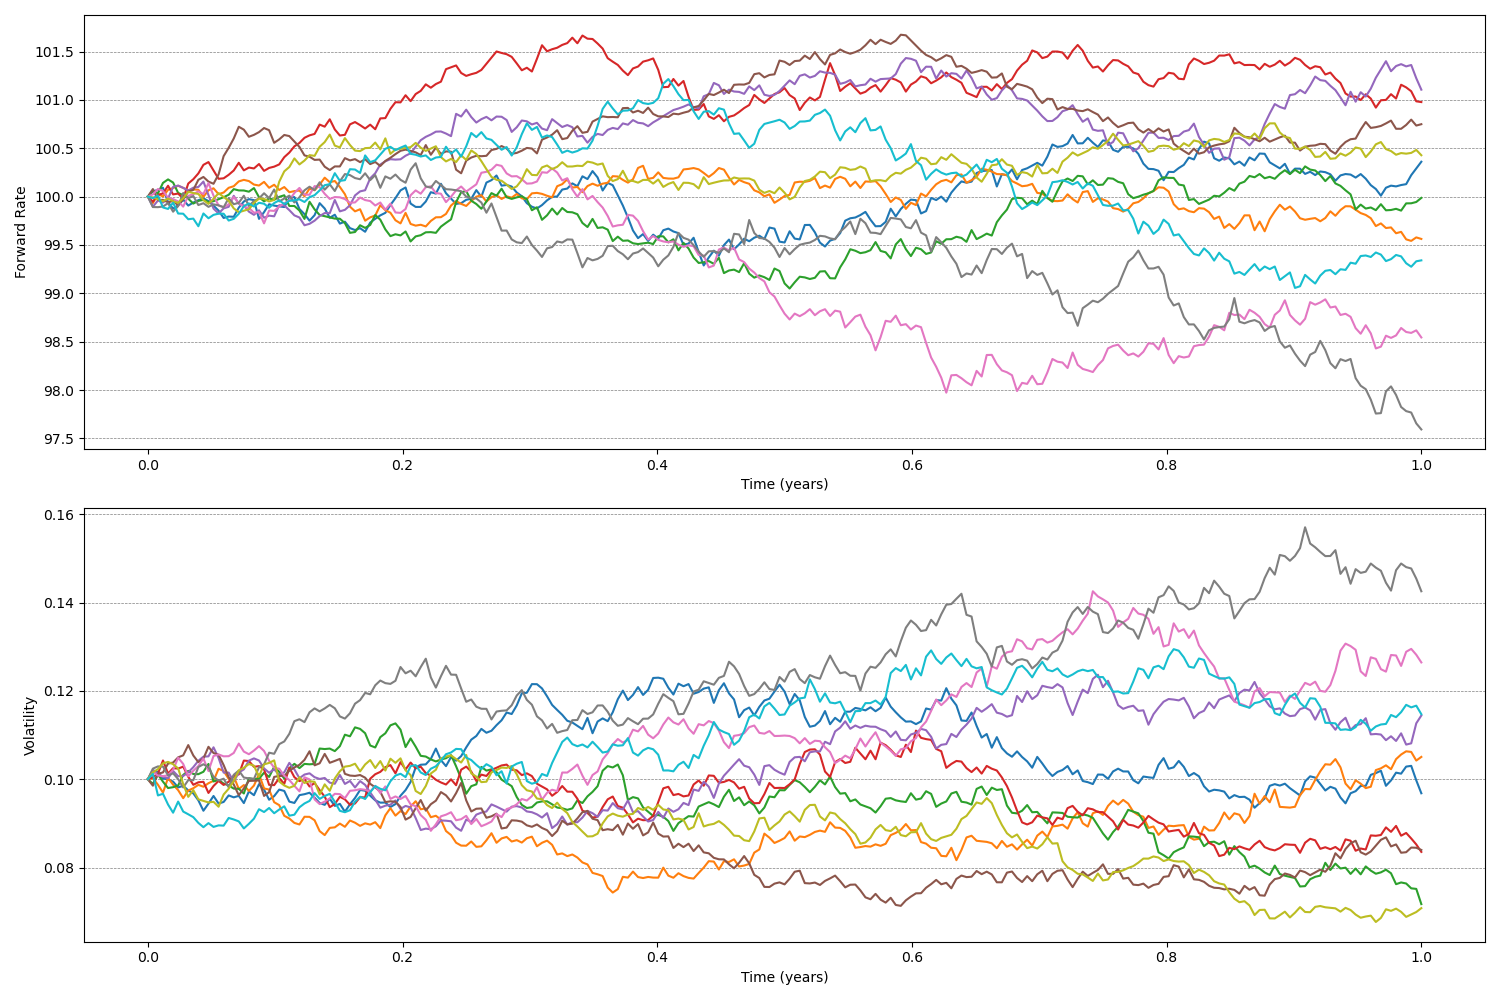
\includegraphics[width=0.8\textwidth]{/Users/nannaingemannohrt/Desktop/master_thesis/main/plots/sim_f_and_sigma.png}
    \caption{Ten simulated paths for the forward rate and the volatility in the SABR model.}
    \label{fig:sim_f_and_sigma}
\end{figure}
\noindent
\subsection{SABR Implied Volatility and Option Prices}
Before we are able to move forward with the analysis,
we need to formulate how to determine implied volatility in the SABR model. 
But these calculations are out of the scope for this analysis,
so we will use the formula in the paper Managing Smile Risk 
of Hagen (2002) \cite{Smile}. The paper states that
under the SABR model, the prices of European options 
is given by Black formula in \autoref{sabr1} to \autoref{sabr3}
below
\begin{align}
    V_{\text{call}} &= D(t_{\text{set}})fN(d_1) - KN(d_2),  \label{sabr1}\\
    V_{\text{put}} &= V_{\text{call}} + D(t_{\text{set}})[K - f], \label{sabr2}
\end{align}
with
\begin{equation}
    d_{1,2} = \frac{\log \frac{f}{K} \pm \frac{1}{2}\sigma_B^2 t_{\text{ex}}}{\sigma_B \sqrt{t_{\text{ex}}}}, \label{sabr3}
\end{equation}
where the implied volatility $\sigma_B(f, K)$ is given by
\begin{equation}
    \sigma_B(K, f) = \frac{\alpha}{(fK)^{(1-\beta)/2}} \left\{ 1 + \frac{(1-\beta)^2}{24} \log^2 \frac{f}{K} + \frac{(1-\beta)^4}{1920} \log^4 \frac{f}{K} + \ldots \right\} \left( \frac{z}{x(z)} \right).
    \label{sigma_B}
\end{equation}
where
\begin{align}
    z &= \frac{\nu}{\alpha}(fK)^{(1-\beta)/2} \log \frac{f}{K}, \\
\end{align}
and x(z) is defined by
\begin{align}
    x(z) &= \log \left\{ \frac{\sqrt{1-2\rho z + z^2} + z - \rho}{1 - \rho} \right\}.
\end{align}
For the special case of at-the-money (ATM) options, options strike at $K = f$, this formula reduces to
\begin{equation}
    \sigma_{ATM} = \sigma_B(f, f) = \frac{\alpha}{f^{1-\beta}} \left\{ 1 + \left( \frac{(1-\beta)^2}{24} \frac{\alpha^2}{f^{2-2\beta}} + \frac{\rho \beta \nu}{4} \frac{\alpha}{f^{1-\beta}} + \frac{2-3\rho^2}{24} \nu^2 \right) t_{\text{ex}} + \ldots \right\}.
    \label{sigma_ff}
\end{equation}
\\
So we have that the parameters $\alpha, \beta, \nu$ and $\rho$  in the SABR model is estimated and the implied volatility $\sigma_B$
is a function of the forward price and the strike. Now that we have a simplified formula for the implied 
volatility from the SABR model, we can start analyzing 
how the model works. We will do this by continuing our
analysis with investigating how the different parameters 
affects implied volatility in the SABR model. 

\subsection{Investigating the parameters of the SABR model}
In this section, we will explore the parameters of the SABR model. This analysis will offer insights into 
how different parameters influence the behavior of implied volatility. We will conduct this investigation using 
the closed-form solution established in the previous section. Our study will be build on  \autoref{sigma_B} and 
\autoref{sigma_ff}, where we will test various parameter values. To see how changes in the different parameters
affects on the implied volatility smile so realistic as possible we fix the values of the parameters.
Below in \autoref{tab:parameters} the chosen values of the parameters are listed, together with a short
explain of the parameters. Then the study is performed by changing the parameters one by one, to illustrate the 
isolated effect of the parameters. 

\begin{table}[H]
    \centering
    \begin{tabular}{ccc}
      \toprule
      \textbf{Parameter} & \textbf{Parameter explanation} & \textbf{Value} \\
      \midrule
      $f$ & Initial forward rate or asset price & 100 \\
      $T$ & Time to maturity & 1 \\
      $K$ & Strike & $K \in (80,120)$ \\
      $\alpha_0$ & Initial level of volatility & 0.1 \\
      $\beta$ & Elasticity of the volatility & 0.5 \\
      $\rho$ & Correlation between the asset price and its volatility & -0.4 \\
      $\nu$ & Volatility of the volatility parameter & 0.25 \\
      \bottomrule
    \end{tabular}
    \caption{Summary of parameters used for investigating the SABR model}
    \label{tab:parameters}
\end{table}
\noindent
We will start the study with investigating how $\alpha_0$ affects the volatility smile in the SABR model. 
First we note that the fixed value of $\alpha_0$ is $0.1$ Hereafter we adjust the value of $\alpha_0$ to $0.05$ and $0.15$,
where the other parameters are kept fixed as listed in \autoref{tab:parameters} above. So having changed the parameter
up and down from the initial value of $\alpha_0$.
We note that the parameter $\alpha_0$
represents "the initial level of volatility" as it is the starting point for the stochastic volatility process. 
Below in \autoref{fig:alpha} the volatility smile is illustrated for three different value of $\alpha_0$. 
From \autoref{fig:alpha} we see that the up and down movements don't change the shape of the volatility smile, 
it only shifts the volatility smile respectively up and down given the movement in $\alpha_0$.
\begin{figure}[H]
    \centering
    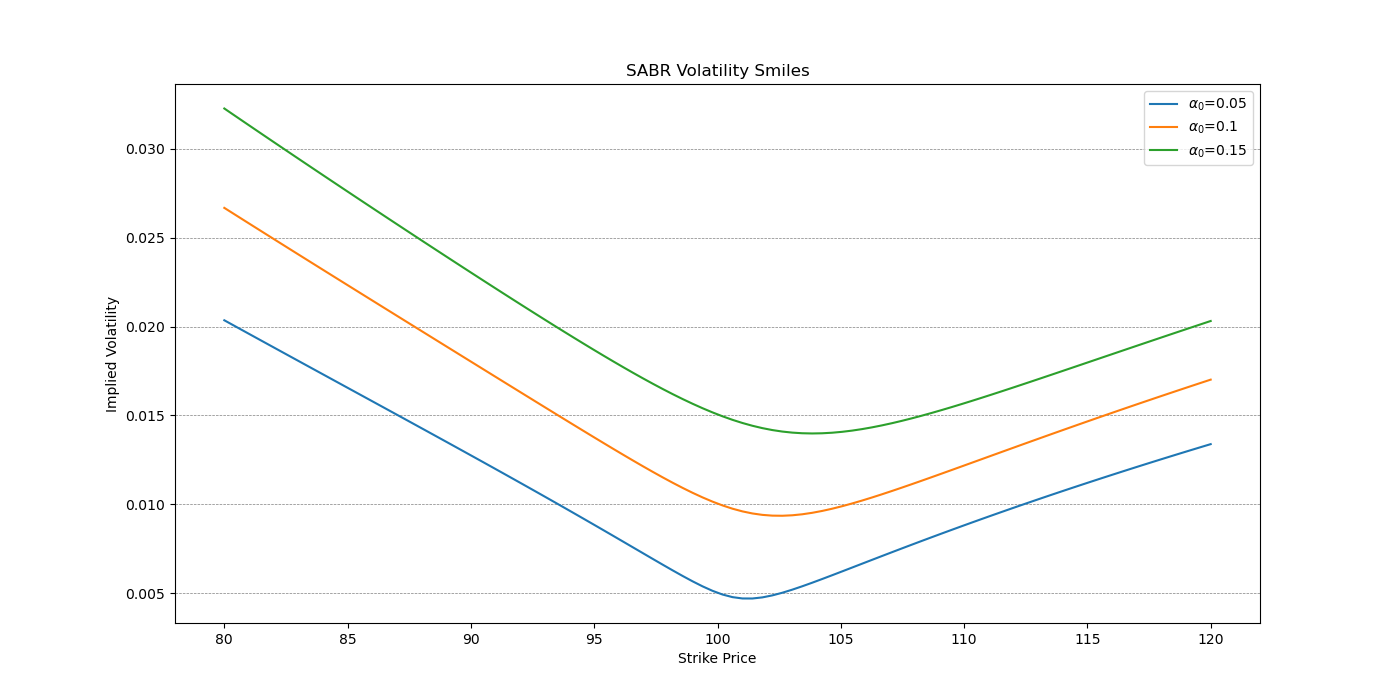
\includegraphics[width=0.7\textwidth]{/Users/nannaingemannohrt/Desktop/master_thesis/main/plots/SABR1_alpha.png}
    \caption{SABR model volatility smiles at various $\alpha_0$ levels}
    \label{fig:alpha}
\end{figure}
\noindent
Then we will continue the study of the parameters affects by looking into shift in the beta value in the SABR model.
Again we shift the value of $\beta$ up and down from the fixed beta in \autoref{tab:parameters}. So we will look at $\beta$ equal to $0.3$,
$0.5$ (the fix beta) and $0.7$. 
Although not explicitly constrained in the original article by Hagan et al. (2002), we restrict $\beta$ to the range $[0, 1]$. 
Choosing a $\beta$ less than 0 would lead to an illogical scenario where higher forward prices F result in a smaller 
relative change in the process $f_t$, thus we set the lower limit at $\beta \leq 0$. Similarly, a $\beta$ greater than 1 would 
suggest that the expected deviation from the current state of $F_t$ exceeds the product of volatility and the current 
forward level (times $\alpha_0 \sqrt{t}$), which is also impractical. Therefore, we set the upper limit at $\beta \geq 1$.
\\\\
Below in \autoref{fig:beta} the volatility smile in the SABR model for the different beta values are illustrated.
From \autoref{fig:beta} we see a small effect of the curvature of the volatility smile. We also note that for higher 
beta the shift is larger, than for lower beta. We also note that the change in the beta parameter is more present in 
the left side from of strike value at-the-money (ATM). Other than that we see the same patterns from the change in 
the alpha parameter, namely the up and down shifts in the volatility smile, respectively to the movement in the 
beta parameter.
\begin{figure}[H]
    \centering
    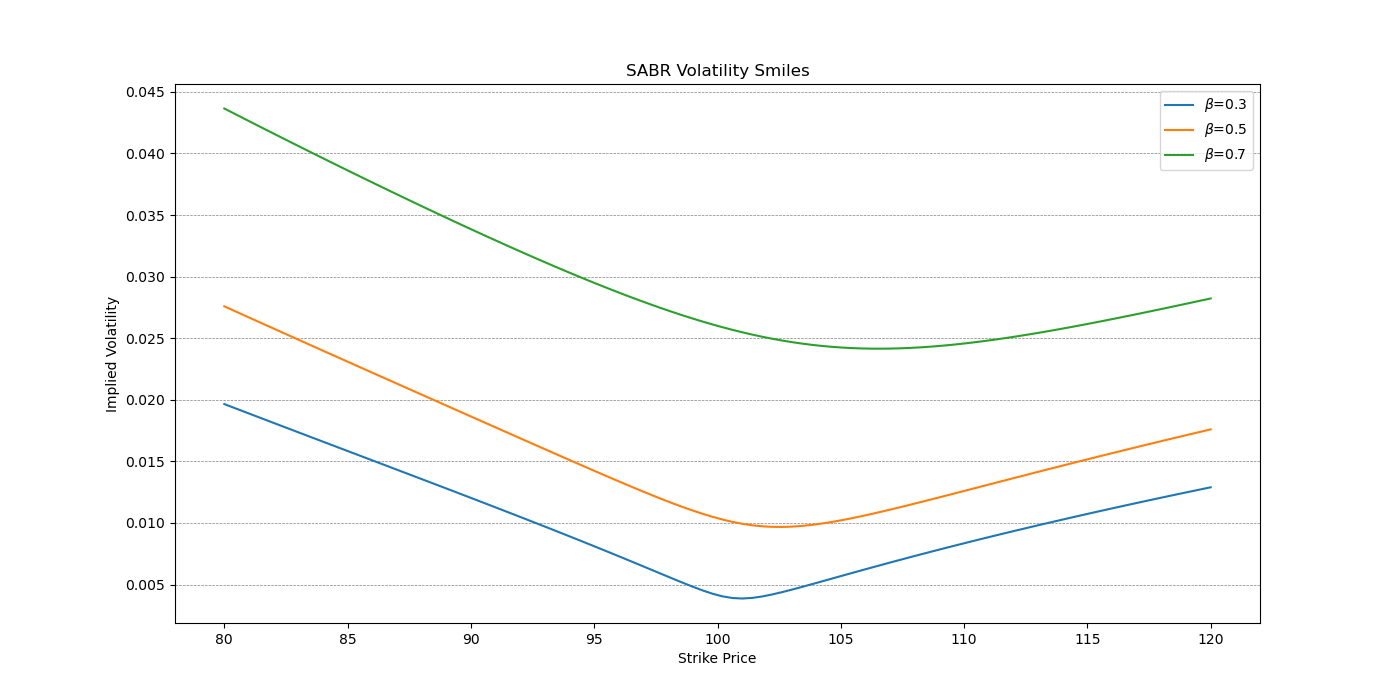
\includegraphics[width=0.7\textwidth]{/Users/nannaingemannohrt/Desktop/master_thesis/main/plots/SABR_beta.png}
    \caption{SABR model volatility smiles at various $\beta$ levels}
    \label{fig:beta}
\end{figure}
\noindent
Moving forward we will shift the $\nu$ parameter, which can be describe as the volatility of the volatility parameter.
Again we shift the $\nu$ parameter up and down from the fixed $\nu$ parameter listed in \autoref{tab:parameters}.
The volatility smile calculated from the SABR for the different $\nu$ parameters are illustrated in \autoref{fig:nu} below.
A very clear pattern emerges, namely that the parameter $\nu$ controls the curvature of the volatility smile in
the SABR model. When we looked at the shifts in the beta parameter we made a comment that it made small changes in 
the curvature. But after this part of the analysis, we clearly see that the curvature is determine from the value
of $\nu$. Which makes sense, when we think of the interpretation of the parameter describe before.
We also note that increasing $\nu$  increased the level of the implied volatility for the 
out-of-the-money (OTM) strikes also increase and vise vera.
\\\\
Then we look at the parameter for the correlation between the asset price and its volatility, namely $\rho$.
So we have that $\rho$ is the correlation between to two Wiener process in the SABR model, note
that $\rho$ is bounded and takes values between $-1$ and $1$. In \autoref{fig:rho} the shifted valus of $\rho$
from the fixed value is illustrated. 
We see that higher positive correlations generally show a decreasing trend in implied volatility with an increase in strike price, 
while strong negative correlations can cause the implied volatility to increase with strikes that are in-the-money (ITM).
We alo note that when the correlation is close to zero the smile is more symmetric around the ATM strike. 
So in total we see that the correlation parameter $\rho$ has a significantly affects on the shape and slope of
the volatility smile in the SABR model, and hence on the implied volatilities values.
\begin{figure}[H]
    \centering
    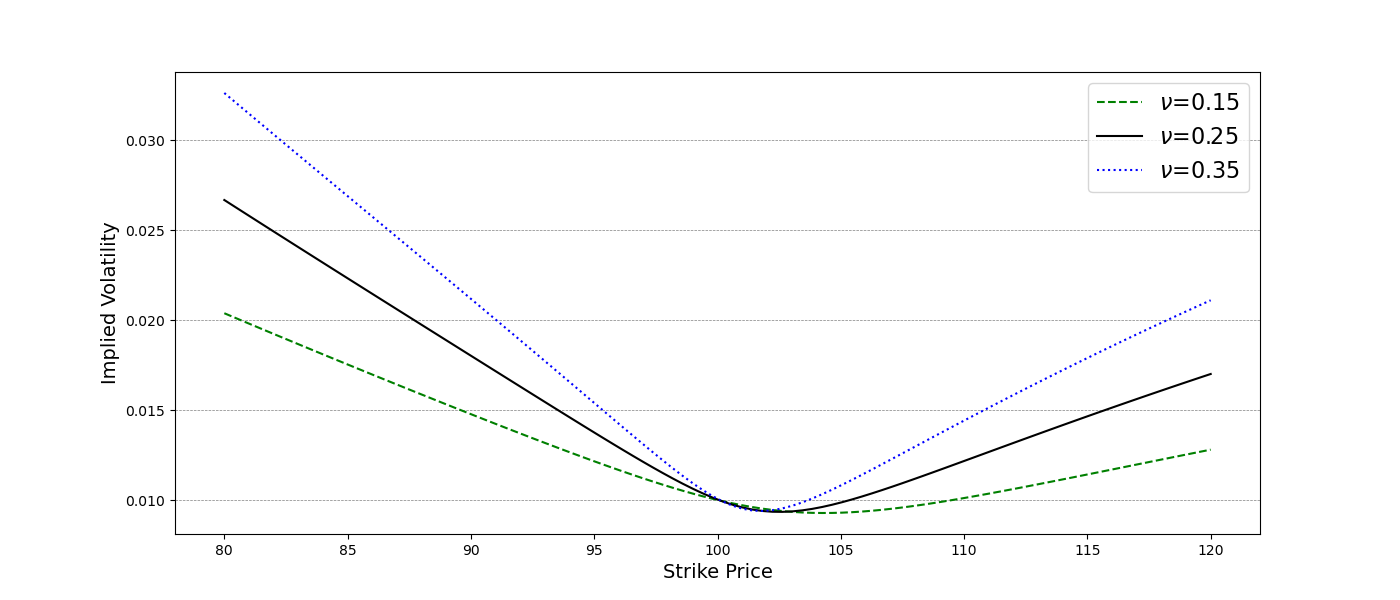
\includegraphics[width=0.7\textwidth]{/Users/nannaingemannohrt/Desktop/master_thesis/main/plots/SABR_nu.png}
    \caption{SABR model volatility smiles at various $\nu$ levels}
    \label{fig:nu}
\end{figure}

\begin{figure}[H]
    \centering
    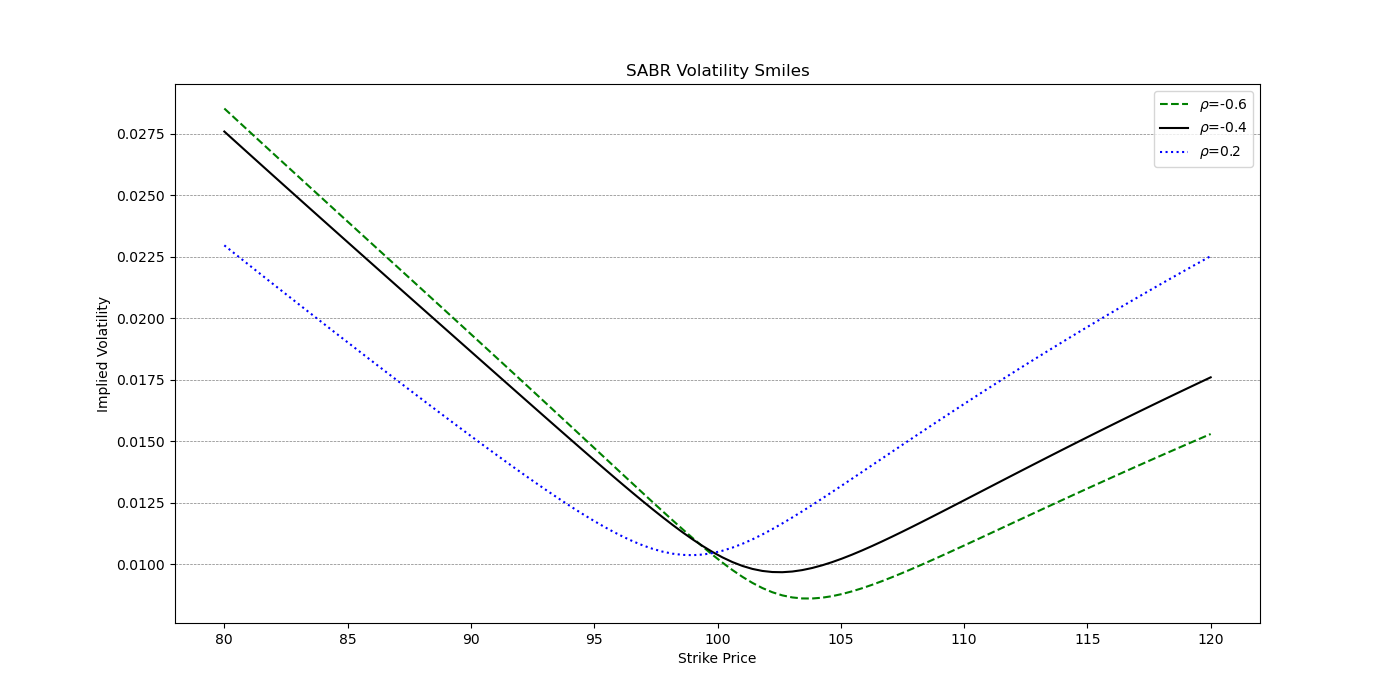
\includegraphics[width=0.7\textwidth]{/Users/nannaingemannohrt/Desktop/master_thesis/main/plots/SABR_rho.png}
    \caption{SABR model volatility smiles at various $\rho$ levels}
    \label{fig:rho}
\end{figure}

\begin{figure}[H]
    \centering
    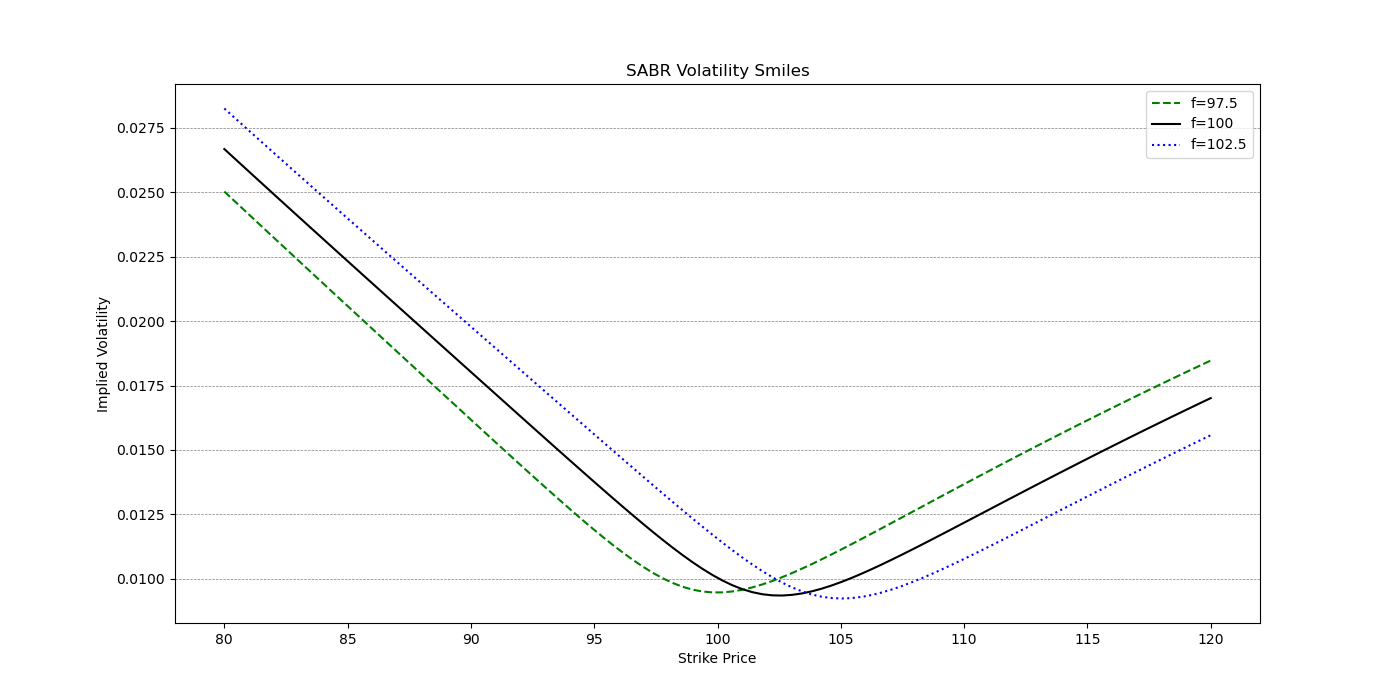
\includegraphics[width=0.7\textwidth]{/Users/nannaingemannohrt/Desktop/master_thesis/main/plots/SABR_f.png}
    \caption{SABR model volatility smiles at various f levels}
    \label{fig:f}
\end{figure}
\noindent
\\\\
Finally we will investigate how the forward price, f, affect the volatility smile in the SABR model. 
The same procedure as for the other parameters will be used. So in \autoref{fig:f} the volatility smile
for the forward prices are illustrated. We see that the slope, shape and curvature is retained, when there
is only change in the forward price. Which is as we expected given how the forward price, f, enters in the closed
solution for the implied volatility in \autoref{sigma_B} and \autoref{sigma_ff}.
\\\\
To summarize this section provides knowledge of the impact of the various parameters in the closed-form solution
for the implied volatility in the SABR model. This knowledge gives a good idea of how that model works, and 
positions us better to understand estimations of the model. So now we have looked at the closed-form solution and 
are ready for the next step of our analysis which is to look at  estimating the parameters in the SABR model.
\newpage
\subsection{Estimating Parameters in the SABR model}
\subsection{Fitting a volatility smile using the SABR model}

\section{Data and the Volatility Risk Premium}

Look at Broekmans

\subsection{Data}

\subsection{The volatility Risk Premium}




\end{document}